%! Author = Axel
%! Date = 21/10/2024

% Preamble
\documentclass[11pt]{article}

% Packages
\usepackage{amsmath}
\usepackage{geometry}
\usepackage{fancyhdr}
\usepackage{titlesec}
\usepackage{hyperref}
\usepackage{graphicx}
\usepackage{float} % Add this line

% Geometry
\geometry{a4paper, margin=1in}

% Header and Footer
\pagestyle{fancy}
\fancyhf{}
\fancyhead[L]{\leftmark}
\fancyhead[R]{\thepage}

% Section formatting
\titleformat{\section}{\large\bfseries}{\thesection}{1em}{}
\titleformat{\subsection}{\normalsize\bfseries}{\thesubsection}{1em}{}

% Document
\begin{document}

\title{Sistemi Operativi Modulo 1 - Appunti}
\author{Axel}
\date{\today}
\maketitle

\tableofcontents
\newpage

\section{I Processi}
\subsection{Requisiti di OS}
Il  Compito fondamentale di un sistema operativo é la gestione dei processi, ovvero delle diverse computazione che si vuol
eseguire su un sistema computerizzato. Il sistema operativo deve:
\begin{itemize}
    \item permettere l'esecuzione alternata di più processi (multitasking)
    \item assegnare le risorse del sistema ai processi, e decidere se dare la CPU a un processo o meno
    \item permettere ai processi di scambiarsi informazioni
    \item permettere la sincronizzazione tra processi (es. semafori)
\end{itemize}
\subsubsection{Cos'è un processo}
Un processo è un programma in esecuzione, ovvero un'istanza di un programma in esecuzione su un computer, un certo programma
puó essere eseguito più volte, e ogni esecuzione è un processo diverso.
L'entitá che puó essere assegnata a un processore è il processo.
Un' unitá di attivitá caratterizzata dall' esecuzione di una sequenza di istruzioni, da uno stato corrente, e da un insieme
associato di risorse di sistema.
un processo è composto da:
\begin{itemize}
    \item Codice
    \item insieme di dati
    \item un numero di attributi che definiscono lo stato del processo
    \end{itemize}
\subsubsection{Processo in escuzione}
processo in esecuzione vuol dire un utente ha richiesto l'esecuzione di un programma, che ancora non é terminato,
ció non significa che il processo sia in esecuzione sulla CPU,decidere se mandare in esecuzione un processo su un
processore é compito del sistema operativo.
Dietro ad ogni processo c'é un programma:
\begin{itemize}
    \item nei sistemi operativi moderni, é solitamente memorizzato su archivio di massa
    \item possono fare eccezzione i processi creati dal sisteme operativo stesso
    \item solo eseguendo un programma si crea un processo
    \item eseguento un programma più volte si creano più processi
\end{itemize}
\subsubsection{Fasi di un processo}
Un processo si compone di 3 macro fasi:
\begin{itemize}
    \item Creazione
    \item Esecuzione
    \item Terminazione
\end{itemize}
La terminazione di un processo può:
\begin{itemize}
    \item essere prevista dal programma
    \item essere non prevista, ad esempio per un errore, in questo caso il sistema operativo lancia una interruzione che puó terminare il processo.
\end{itemize}
\subsubsection{Elementi di un processo}
Finché il processo é in esecuzione, il sistema operativo deve tener traccia di:
\begin{itemize}
    \item Identificatore del processo
    \item Stato del processo (Runing,...)
    \item Priorità del processo
    \item Hardware Context: valore corrente dei registri del processore (include program counter)
    \item puntatori alla memori (definisce l'immagine del processo)
    \item informazioni sullo stato dell'input/output
    \item informazioni di accounting (quale utente lo esegue)
\end{itemize}
\subsection{Process Control Block}
Il sistema operativo mantiene un Process Control Block (PCB) per ogni processo, che contiene tutte le informazioni necessarie,
che sono contenute nella zona di memoria riservata al kernel, solo il sistema operativo può accedere a queste informazioni.
consente al sistema operativo di gestire piú processi contemporaneamente, contiene sufficiente informazioni per permettere
al sistema operativo di sospendere un processo e riprenderlo in un secondo momento.
\subsection{Traccia di un processo}
Il comportamento di un particolare processo é determinato dalla sequenza di istruzioni che esegue, e dallo stato del processo,
questá sequenza é detta trace, il \textbf{Dispatcher} é un piccolo programma che sospende un processo per farne andare in esecuzione un altro
\subsection{Eseuzione di un processo}
Considerando 3 processi, Ogni processo viene eseguito senza interruzzioni fino al termine, ma in veritá il dispatcher
sospende un processo per farne eseguire un altro, il tempo di esecuzione di un processo é diviso in piccoli intervalli
di tempo, detti \textbf{time slice} es :
\begin{itemize}
    \item Parte il processo A
    \item dopo un certo tempo il dispatcher sospende il processo A e fa partire il processo B
    \item dopo un certo tempo il dispatcher sospende il processo B e fa partire il processo C
    \item dopo un certo tempo il dispatcher sospende il processo C e fa partire il processo A
    \item e cosí via
    \item il dispatcher é un programma che si occupa di fare questo
\end{itemize}
\subsection{Modello dei Processi a 2 stati}
Un processo può essere in uno di due stati:
\begin{itemize}
    \item Running: il processo é in esecuzione sulla CPU
    \item Not Running: il processo é in attesa di essere eseguito
\end{itemize}
esitono anche 2 stati nascosti ovvero: entrante e uscente, in ogni caso é il dispatcher che si occupa di fare il cambio di stato tra Running e not Running
Dal punto di vista dell'implementazione esiste una coda di processi pronti, il dispatcher prende il primo processo dalla coda e lo esegue sulla CPU
\subsection{Creazione di un processo}
In ogni istante ci sono n>=1 processi in esecuzione, come minimo c'é un interfaccia GUI,...ecc
Se l'utente dá un comeando quasi sempre si crea un processo, la creazione di un processo avviene con il
\textbf{Process Spawning}: un processo crea un altro processo, il processo che crea il processo é detto \textbf{parent process}, il processo creato é detto \textbf{child process},
in questa maniera si crea una gerarchia di processi, il processo padre puó creare più processi figli, e un processo figlio puó creare altri processi figli.
\subsection{Terminazione di un processo}
Un processo puó terminare in 2 modi:
\begin{itemize}
    \item Normale completamento: istruzione macchina HALT, che generi un'interruzione per OS, in linguaggi di alto livello l'istruzione HALT é invocata da una system call come exit inserita dai compilatori
    \item Kill: Il sistema operativo puó terminare un processo in modo forzato, per errori come:
    \begin{itemize}
        \item Memoria non disponibile
        \item Errore di protezione
        \item Errore fatale a livello di istruzione(Divisione per 0)
        \item operazione di I/O fallita
        \end{itemize}
    oppure l'utente puó terminare un processo con un comando
    \end{itemize}
    si passa quidi da n >= 2 processi a n-1 processi
    C'é sempre un processo master che non puó essere terminato, il processo master é il primo processo che viene eseguito
\subsection{Modello dei processi a 5 stati}
il modello a 2 stati é troppo semplice, il modello a 5 stati é più realistico, un processo puó essere in uno di 5 stati:
\begin{itemize}
    \item New: il processo é stato creato ma non é ancora in esecuzione
    \item Ready: il processo é pronto per essere eseguito
    \item Running: il processo é in esecuzione sulla CPU
    \item Blocked: il processo é in attesa di un evento (es. I/O)
    \item Terminated: il processo é terminato
    \end{itemize}
le transizioni tra gli stati sono:
\begin{itemize}
    \item New $\rightarrow$ Ready: il processo è stato creato e pronto per essere eseguito
    \item Ready $\rightarrow$ Running: il processo è in esecuzione sulla CPU
    \item Running $\rightarrow$ Ready: il processo è stato sospeso
    \item Running $\rightarrow$ Blocked: il processo è in attesa di un evento
    \item Blocked $\rightarrow$ Ready: il processo è pronto per essere eseguito
    \item Running $\rightarrow$ Terminated: il processo è terminato
\end{itemize}
\begin{figure}[h]
    \centering
    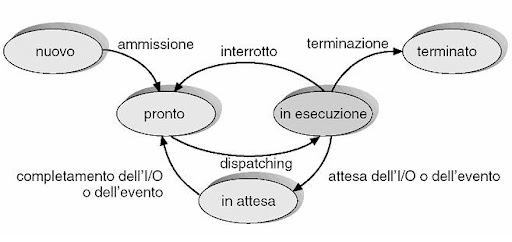
\includegraphics[width=0.5\textwidth]{immagini/processo a 5 stati}
    \caption{Modello dei processi a 5 stati}
\end{figure}
Cosa c' é dietro a blocked ? il processo é in attesa di un evento, es. I/O, il processo é sospeso e il sistema operativo
si occupa di far partire un altro processo, quando l'evento é completato il processo torna in ready. il dispatcher per cui
non metterá mai un processo blocked in esecuzione.
Con 5 stati abbiamo bisogno quindi 2 code di processi:
\begin{itemize}
    \item Ready Queue: contiene i processi pronti per essere eseguiti
    \item Blocked Queue: contiene i processi in attesa di un evento
\end{itemize}
I sistemi operativi hanno piú di una coda di eventi che contiene gli eventi che devono essere completati, quando un evento é completato
il processo torna in ready
\begin{figure}
    \centering
    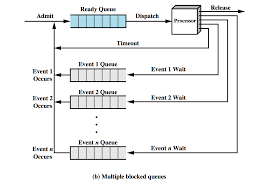
\includegraphics[width=0.5\textwidth]{immagini/5StatiCode2}
    \caption{Diagramma delle 2 code di processi}
\end{figure}
\subsection{Processi Sospesi}
Esiste la possibilitá di avere dei processi sospesi, questo é dovuto quando molti processi sono in attesa di un evento,
quindi fino a che sono bloccati non possono essere eseguiti, quindi vengono spostati dalla RAM al disco, in questo modo
si libera spazio in RAM, quando l'evento é completato il processo viene spostato dalla memoria secondaria alla RAM,
questo cambiamento aggiunge 2 stati ai 5 precedenti:
\begin{itemize}
    \item Ready Suspended: il processo é pronto per essere eseguito ma é sospeso
    \item Blocked Suspended: il processo é in attesa di un evento ma é sospeso
\end{itemize}
\begin{figure}
    \centering
    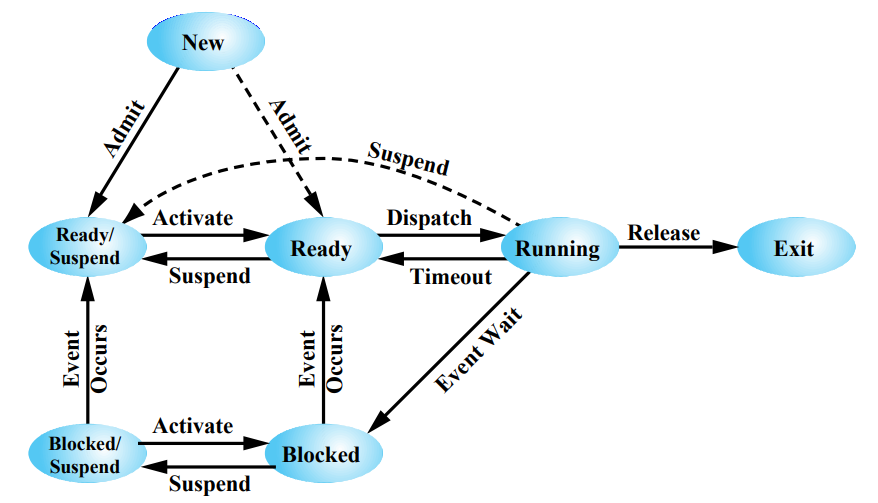
\includegraphics[width=0.5\textwidth]{immagini/7State}
    \caption{Modello dei processi a 7 stati}
\end{figure}
I motivi per sospendere un processo sono:
\begin{itemize}
    \item Swapping: il processo é spostato dalla RAM al disco
    \item Interno al OS : Il sistema sospetta che il processo stia causando problemi
    \item Periodicitá: il processo viene eseguito solo periodicamente
    \item Richiesta del processo padre : il processo padre puó richiedere di sospendere un processo figlio
\end{itemize}
\subsection{Strutture di controllo del OS}
Il sistema operativo é l'entitá che si occupa di gestire le risorse da parte dei processi,
per fare ció esso deve conoscere lo stato di ogni processo, per compiere questa operazione il sistema operativo
crea 1 o piú tabelle
\begin{figure}
    \centering
    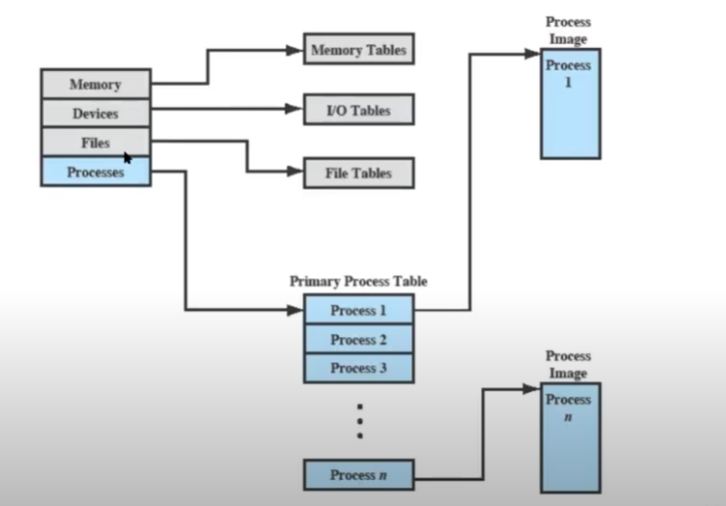
\includegraphics[width=0.5\textwidth]{immagini/ControlTable}
    \caption{Strutture di controllo del OS}
\end{figure}
per ciascuna delle risorse esistono tabelle per gestire la memoria, i file, i dispositivi di I/O e i processi
tutte queste tabelle si trovano nella zona di memoria riservata al kernel
\subsubsection{Memory Table}
Le tabelle di memoria sono usate per gestire sia la memoria principale che quella secondaria(quella secondaria serve per la memoria virtuale),
le tabelle di memoria contengono informazioni su:
\begin{itemize}
    \item allocazione di memoria principale da parte dei processi
    \item allocazione di memoria secondaria da parte dei processi
    \item attributi di protezione per l'accesso a zone di memoria
    \item informazioni per gestire la memoria virtuale
\end{itemize}
\subsubsection{Tabelle per l'I/O}
Le tabelle per l'I/O contengono informazioni su:
\begin{itemize}
    \item se il dispositivo é disponibile o giá assegnato
    \item lo stato dell'operazione di I/O
    \item la locazione in memoria principale usata come sorgente o destinazione dell'operazione di I/O
\end{itemize}
\subsubsection{File Table}
Le tabelle per i file contengono informazioni su:
\begin{itemize}
    \item Esistenza di un file
    \item Locazioni in memoria secondaria
    \item Stato corrente
    \item Altri attributi
\end{itemize}
\subsubsection{Process Table}
Per gestire i processi il sistema operativo usa una tabella di processi, che contiene informazioni su:
\begin{itemize}
    \item Stato del processo
    \item identificatore del processo
    \item locazione in memoria
\end{itemize}
Blocco di controllo dell'processo (PCB) é un blocco di informazioni che contiene tutte le informazioni necessarie per gestire un processo
\newline
Si dice \textbf{process image} l'insieme di programma sorgente,dati,stack delle chiamate e PCB, eseguire un'istruzione cambia l'immagine
, unica possiblie eccezzione é l'istruzione di jump all'istruzione stessa.
\subsection{Attributi di un processo}
Le informazioni in ciascun bloocco di controllo del processo possono essere raccolte in 3 gruppi:
\begin{itemize}
    \item Identificazione
    \item Stato
    \item Controllo
\end{itemize}
\subsubsection{Come si Identifica un processo}
ad ogni processo é assegnato un identificatore unico, che é un intero positivo, Molte tabelle del OS usano PID
per realizzare collegamenti tra le varie tabelle.
\subsubsection{Stato del processore}
Da non confondere con lo stato del processo, é dato dai contenuti dei registri del processore stesso:
\begin{itemize}
    \item registri visibili all'utente
    \item registri di controllo e di stato
    \item puntatori allo stack
    \item PSW(Program Status Word) : la program status word contiene informazioni sullo stato del processo
    \end{itemize}
\subsubsection{Control Block del Processo}
Per Ricapitolare il PCB contiene:
\begin{itemize}
    \item Contiene informazioni di cui l'OS ha bisogno per coordinare processi attivi
    \item Identificatori : PID, PPID (parent process ID) oppure dell'utente che lo ha eseguito
    \item Informazioni sullo stato del processore : registri utente, program counter, stack pointer e registri di stato
    \item Informazioni per il controllo del processo : priorità, stato del processo, informazioni di scheduling, l'evento d'attender per essere ready
    \item Supporto per strutture dati: puntatori ad altri processi, per fare code di processi o liste di processi
    \item Comunicazione tra processi: informazioni per la comunicazione tra processi flag,segnali,messaggi
    \item Permessi Speciali: permessi speciali per l'accesso a risorse
    \item Gestione della memoria: puntatori ad aree di memoria
    \item Gestione delle Risorse : file aperti, ecc.
\end{itemize}
\subsection{Processi e Memoria virtuale}
Se ci sono n processi attivi, ci sono n PCB, e sono conservati nella ram conservati nella zona del kernel, tutto il
resto é conservato nella memoria virtuale, una parte della memoria virtuale puó essere condivisa tra i processi mentre
normalmente un processo non puó accedere alla memoria di un altro processo é peró possibile
condividere la memoria se chi ha scritto il programma lo ha previsto, es. condividere una variabile tra 2 processi.
Tutto questo fa si che il control block sia una delle strutture dati piú importanti del sistema operativo perché definisce lo stato dell'OS stesso,
Richiede inoltre Protezione, una funzione scritta male potrebbe danneggiare il blocco.
\subsection{Modalita di esecuzione}
La maggior parte dei processori supporta almeno due modalitá di esecuzione:
\begin{itemize}
    \item Modalitá utente: molte operazioni non sono permesse
    \item Modalitá kernel : pieno controllo del processore ad esempio si possono eseguire istruzione macchina
\end{itemize}
\subsubsection{Kernel Mode}
Il kernel mode é la modalitá di esecuzione in cui il sistema operativo ha il controllo completo del processore,
si possono gestire i processi (tramite PCB)
\begin{itemize}
    \item creazione e terminazione di processi
    \item pianificazione di lungo,messo e corto termine(scheduling e dispatching)
    \item avvicendamento dei processi(switching)
    \item sincronizzazione e comunicazione tra processi
\end{itemize}
si puó gestire la memoria principale:
\begin{itemize}
    \item allocazione di spazio
    \item gestione della memoria virtuale
\end{itemize}
si puó gestire l'I/O:
\begin{itemize}
    \item gestione dei buffer e delle cache per l'I/O
    \item assegnazione risorse I/O ai processi
\end{itemize}
Funzioni Supporto: Gestione interrupt/eccezzioni,accounting,monitoraggio
\subsubsection{Da UserMode a KernelMode}
Esite quindi la necessita di passare da user mode a kernel mode, esempio: un processo vuole fare una operazione di I/O,
deve chiedere il permesso al sistema operativo, di passare in kernel mode, per poi tornare in user mode.
Ogni processo inizia sempre in user mode, se viene fatta una richiesta che necessita della kernel mode come una system call
il processo passa in kernel mode, il sistema operativo esegue la system call e poi torna in user mode, l'ultima istruzione
dell'interrupt handler é una istruzione di ritorno che fa tornare il processo in user mode.
esistono quindi 3 casi in cui si passa in kernel mode:
\begin{itemize}
    \item Codice eseguito per conto dello stesso processo interrotto, che lo ha esplicitamente voluto
    \item Codice eseguito per conto dello stesso processo interrotto, che non lo ha esplicitamente voluto
    \item Codice eseguito per conto di un altro processo
\end{itemize}
Esempio di system call sui pentium:
\begin{enumerate}
    \item prepara gli argomenti della chiamata nei registri, tra tali argomenti c'é un numero che identifica la system call
    \item esegue lístruzione int 0x80, che appunto solleva un interrupt(in realtá una eccezzione)
    \end{enumerate}
Anche creare un nuovo processo é una system call : l'handler di questa system call verrá ovviamente eseguito in modalitá kernel,puó quindi modificare la lista dei PCB
\subsection{Creazione del processo}
per creare un processo il sistema operativo deve:
\begin{itemize}
    \item Assegnargli un PID Unico
    \item Allocargli spazio in memoria principale
    \item Inizializzare il PCB
    \item Inserire il processo nella giusta coda
    \item Creare o espandere strutture dati
\end{itemize}
\subsection{Switching tra processi}
Lo switching tra processi é il passaggio da un processo all'altro, ovver per qualche motivo l'attuale processo non deve piú usare
il processore che concesso ad un altro processo.
\subsubsection{Quando effettuare lo switching}
Lo switching tra processi puó avvenire per diversi motivi:
\begin{itemize}
    \item interruzzione : Cause esterna all'esecuzione dell'istruzione corrente Uso Reazione a un evento esterno asincrono, include i quanti di tempo per lo scheduler
    \item Eccezzione: Associata all'esecuzione dell'istruzione, gestione di un errore sincrono
    \item Chiamata al OS : Richiesta esplicita, chiamata a funzione di sistema
\end{itemize}
\subsubsection{Passaggi per lo switching}
\begin{enumerate}
    \item Salvare il contesto del programma (registri e PC) salvati nel PCB
    \item Aggiornare il process control block, attualmente in running
    \item Spsotare il PCB nella coda appropriata : ready,blocked;ready/suspended
    \item Scelgiere un nuovo processo da eseguire
    \item Aggiornare il process control block del processo selezionato
    \item Aggiornare le strutture dati per la gestione della memoria
    \item Ripristinare il contesto del processo selezionato
\end{enumerate}
\subsubsection{Il Sistema operativo é un processo}
Il sistema operativo é un insieme di programmi, ed é eseguito dal processore come ogni altro programma, semplicemente
lascia che altri programmi vadano in esecuzione, per poi riprendere il controllo tramite interrupt, quindi se é un processo lui stesso
deve essere gestito...
esistono quinndi 3 modi per gestire il sistema operativo:
\begin{itemize}
    \item kernel separato : il sistema operativo é un processo separato
    \item kernel unico : il sistema operativo é un processo come gli altri
    \item Sistemi ibridi : il sistema operativo é un processo separato, ma esiste un kernel unico
\end{itemize}
\subsubsubsection{Kernel non é un processo}
il kernel é eseguito al di fuori dei processi, il concetto di processo si applica solo ai processi utente, il kernel é eseguito
\subsubsubsection{Esecuzione all'interno dei processi utenti}
Il SO viene eseguito nel contesto di un processo utente, non c'é bisogno di un process switch per eseguire una funzione del sistema operativo,
sole del mode switch, Comunque , stack delle chiamate separato, process switch solo,eventualmente, per passare il controllo ad un altro processo
\subsubsubsection{Sistema Basato su processi}
il sistema operativo é un insieme di processi, ogni processo é un modulo del sistema operativo, ogni processo é un modulo del sistema operativo,
ogni processo partecipa alla competizione per il processore, lo switch peró non é un processo
\subsubsection{Esempio in Linux}
In linux ci sono peró anche dei processi di sistema, che partecipano alla normale competizione per il processore, senza essere invocati esplicitamente,
sono operazioni tipiche del sistema operativo, es. gestione della memoria, gestione dei dispositivi di I/O
\begin{figure}
    \centering
    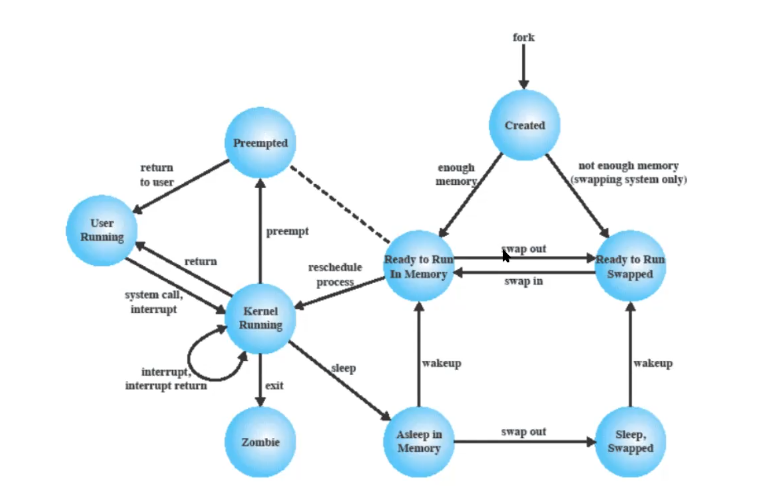
\includegraphics[width=0.75\textwidth]{immagini/transizioneTraStatiDeiProcessi}
    \caption{Diagramma stati Unix}
\end{figure}
\subsubsection{Stati in Unix}
Con l'istruzione fork() si crea un processo figlio,
una volta che il processo é stato creato, abbiamo 2 possibili stati Run in memory oppure Run in swapped(Memoria Virtuale)
i due stati sono intercambiabili ovvero posso spostare il processo dalla memoria principale alla memoria virtuale e viceversa
anche lo stato di sospensione puó avvenire in memoria o in memoria virtuale. Quando il processo in running si trova in user mode
, quando vengono effettuate delle system call il processo passa in kernel mode, quando siamo in kernel mode c'é la possibilitá di
effettuare la preemption, ovvero sospendere il processo per farne eseguire un altro, il processo puó essere sospeso per un interrupt
, nello stato di preemption si prende in considerazione l'idea di non continuare l'esecuzione, quando un processo finisce va
nello stato zombie (Tipico dei sistemi Unix), quello che succede é che ci si aspetta che il processo padre soppravviva al figlio
e fino a che il processo figlio non comunica al padre che ha terminato, il processo figlio rimane nello stato zombie, l' unica cosa
che rimane é il PCB, quando il processo padre comunica al sistema operativo che il processo figlio é terminato, il processo figlio.
\subsubsection{Transizione tra processi}
non é interrompibile quando siamo in kernel mode quindi non va bene per sistemi real time
\subsection{Immagine del processo in Unix}
Un insieme di strutture dati forniscono al sistema operativo le informazioni necessarie per gestire un processo
\begin{itemize}
    \item User Area : contiene il codice, i dati e lo stack del processo
    \begin{enumerate}
        \item \textbf{Codice}: linguaggio macchina
        \item \textbf{Dati}: variabili globali e locali
        \item \textbf{Stack}: contiene le informazioni necessarie per gestire le chiamate a funzione
        \item \textbf{Memoria Condivisa}: usata per la comunicazione tra processi (deve essere esplicitamente richiesta)
    \end{enumerate}
    \item Registro : contiene i registri del processore
    \begin{enumerate}
        \item \textbf{Program Counter}: contiene l'indirizzo dell'istruzione corrente
        \item \textbf{Stack Pointer}: contiene l'indirizzo della cima dello stack
        \item \textbf{Registri Generali}: contengono i dati temporanei
    \end{enumerate}
    \item sistema : contiene le informazioni necessarie per la gestione del processo a livello di memoria
    \begin{enumerate}
        \item \textbf{Process Table Entry}: puntatore alla tabella di tutti i processi, dove individua quello corrente
        \item \textbf{U Area}: informazioni per il controllo dell'processo, informazioni addizzionali per quando il kernel viene eseguito da questo processo
        \item \textbf{Per process region table}: definisce il mapping tra indirizzi logici e fisici (Page Table), inoltre indica se per questo processo tali indirizzi sono in lettura, scrittura o esecuzione
        \item \textbf{Kernel Stack}: Stack delle chiamate, separato da quello utente, usato per le funzioni da eseguire in modalitá sistema (kernel mode)
    \end{enumerate}
\end{itemize}
\begin{table}[H]
    \raggedright
    \begin{tabular}{|c|p{10cm}|}
        \hline
        Process Status & Current State \\
        \hline
        Pointers & puntatori alle zone del processo\\
        \hline
        Process Size & quanto é grande l' immagine del processo (il PCB ha una grandezza predefinita) \\
        \hline
        User Identifier & Identificatore dell'utente che ha lanciato il processo, c'é una differenza tra \textbf{Real User ID} e \textbf{ effective user ID}  \\
        \hline
        Process ID & Identificatore del processo \\
        \hline
        Event Descriptor & Motivazioni per il quale il processo é bloccato \\
        \hline
        Priority & Prioritá del processo \\
        \hline
        Signal State & Stato dei segnali \\
        \hline
        Timers & Include il tempo di esecuzione del processo, l'utilizzo delle risorse del kernel, timer usati per mandare segnali di allarme ad un processo \\
        \hline
        P_Links & Puntatori per le code di processi(LinkedList), \\
        \hline
        Memory Status & Indicazioni se la memoria é in memoria principale o secondaria, indica anche se il processo se puó essere spostato \\
        \hline
    \end{tabular}
    \caption{Process Table entry}
    \label{tab:esempio}
\end{table}
\section{I Thread}
Ci sono alcune applicazioni che richiedono la gestione in parallelo, ovvero quando viene programmata un'applicazione
viene suddivisa in piú parti, quindi l'applicazione rimane un singolo processo, ma che al suo interno esegue
piú computazioni in parallelo, quindi possiamo dire che un processo puó essere composto da piú thread.
In questo caso é compito del programmatore occuparsi della sincronizzazione tra i thread, il sistema operativo
si occupa di gestire i processi, mentre il programmatore si occupa di gestire i thread.
Diversi thread condividono molte risorse, del processo, non condividono lo stack delle chiamate ed anche il processore,
condividono invece memoria(Stack Esclusi), files, dispositivi di I/O, ecc.
Teoricamente si puó dire che il processo incorpori gestione delle risorse e scheduling
\begin{figure}[H]
    \centering
    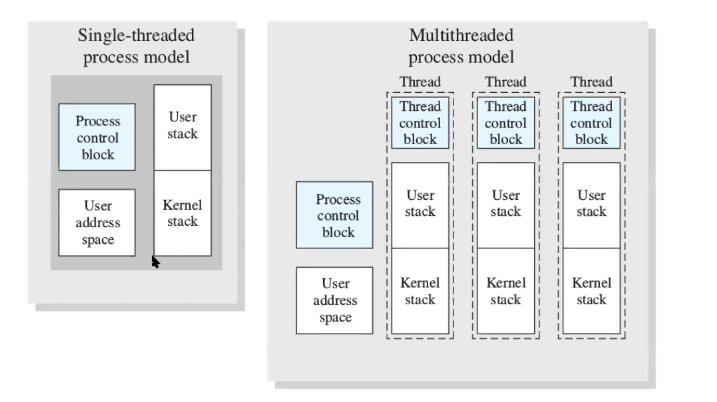
\includegraphics[width=0.5\textwidth]{immagini/thread1}
    \caption{Thread}
\end{figure}
Se sono su un sistema operativo Single Threaded, il sistema operativo non supporta il multithreading, ho l'immagine del processo
ed il PCB, se il sistema operativo supporta il multithreading, ho l'immagine del processo, il PCB e il TCB(Thread Control Block),
dove Il TCB gestisce solo la parte dello scheduling
\subsection{Perché introdurre i thread}
Creare un thread é semplice/efficiente, la creazione la terminazione, fare lo switching e farli comunicare,
quindi ogni processo viene creato con un thread, dopo il programmatore puo' creare altri thread con il comando spawn()
, esistono chiamate di sistema per bloccare un thread, sbloccare un thread, terminare un thread.
\subsection{ULT e KLT}
Esistono 2 tipi di thread:
\begin{itemize}
    \item ULT(User Level Thread): A livello di sistema operativo i thread non esistono, oppurtune librerie si occupano di gestire il thread
    \item KLT(Kernel Level Thread): Il sistema operativo supporta i thread, quindi il sistema operativo é a conoscenza dei thread
    \item
\end{itemize}
\begin{figure}[H]
    \centering
    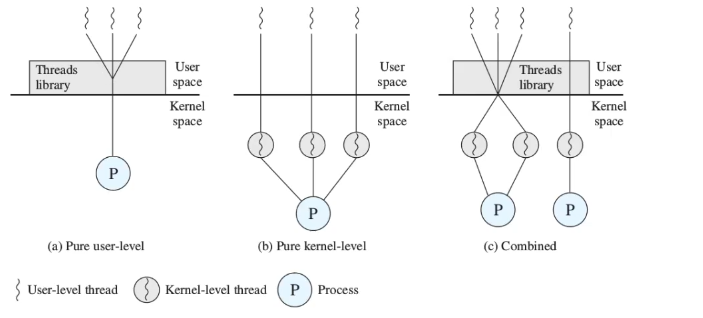
\includegraphics[width=0.5\textwidth]{immagini/ULTeKLT}
    \caption{ULT e KLT}
\end{figure}
perché usare ULT:
\begin{itemize}
    \item Sono piú veloci da creare e gestire (Non serve fare il mode swithcing)
    \item Si puó avere una politica di scheduling per ogni processo
    \item Permettono di usare i thread anche sui sistemi operativi che non li offrono nativamente
\end{itemize}
perché NON usare ULT:
\begin{itemize}
    \item Se un thread si deve bloccare, si bloccano tuitti i thread del processo, a meno che il blocco non sia chiamato
    dalla chiamata di block, al contrario con i KLT solo il thread che si blocca viene bloccato
    \item Se ci sono piú processori o piú core, i thread non possono essere eseguiti in parallelo perché il sistema operativo
    non é a conoscenza dei thread
\end{itemize}
\subsection{Processi e Thread in Linux}

I thread sono spesso associati al termine Light Weight Processes o LWP. Questo termine risale ai tempi in cui Linux supportava i thread solo a livello utente. Ciò significa che anche un'applicazione multithread era vista dal kernel come un singolo processo. Questo creava grandi sfide per la libreria che gestiva questi thread a livello utente, poiché doveva garantire che l'esecuzione di un thread non fosse ostacolata se un altro thread emetteva una chiamata bloccante.

Successivamente l'implementazione è cambiata, e ai processi sono stati collegati singoli thread, in modo che fosse il kernel a gestirli. Tuttavia, come discusso in precedenza, il kernel Linux non li vede come thread: ogni thread è trattato come un processo all'interno del kernel. Questi processi sono conosciuti come processi leggeri o light weight processes.

La principale differenza tra un processo leggero (LWP) e un processo normale è che gli LWP condividono lo stesso spazio di indirizzamento e altre risorse come i file aperti. Poiché alcune risorse sono condivise, questi processi vengono considerati più "leggeri" rispetto agli altri processi normali, da cui il nome di processi leggeri.

Quindi, in sostanza, possiamo dire che thread e processi leggeri sono la stessa cosa. È solo che thread è un termine usato a livello utente, mentre light weight process è un termine utilizzato a livello di kernel.


Nel kernel, ogni thread ha il proprio ID, chiamato PID (anche se forse avrebbe più senso chiamarlo TID), e ha anche un TGID (Thread Group ID) che corrisponde al PID del thread che ha avviato l'intero processo.

Semplificando, quando viene creato un nuovo processo, appare come un thread in cui sia il PID che il TGID sono lo stesso nuovo numero.

Quando un thread avvia un altro thread, il thread avviato ottiene il proprio PID (in modo che lo scheduler possa programmarlo indipendentemente), ma eredita il TGID dal thread che lo ha creato.

In questo modo, il kernel può programmare i thread indipendentemente dal processo a cui appartengono, mentre i processi (gli ID del gruppo di thread, o TGID) vengono mostrati agli utenti.

Per ogni thread, esiste quindi un PCB per ogni thread, questo crea un piccolo overhead perché esiste una duplicazione di alcune informazioni(puntatori)
\subsection{Gli stati dei processi in Linux}
Linux ha 5 stati per i processi, linux non distingue tra ready e running, divide peró in due stati blocked,
\begin{itemize}
    \item Task Running: il processo é in esecuzione sulla CPU
    \item Blocked:
    \begin{enumerate}
        \item Task Interruptible: il processo é in attesa di un evento, ma puó essere interrotto
        \item Task Uninterruptible: il processo é in attesa di un evento, ma non puó essere interrotto
        \item Task Stopped: il processo é stato fermato
        \item Task Traced: il processo é tracciato
    \end{enumerate}
    \item EXIT Zombie: il processo é terminato, ma il processo padre non ha ancora comunicato al sistema operativo
    \end{itemize}
\subsection{Segnali ed interrupt in Linux}
Non bisogna confondere i segnali con gli interrupt, I segnali possono essere inviati da un processo ad un altro processo,
quello che succede che il campo del PCB viene aggiornato con il segnale che é stato inviato, quando il processo
viene schedulato, il kernel controlla se ci sono segnali da gestire se si esegue la funzione di gestione del segnale,
alcuni signa handlers possono essere sovrascritti dal programmatore, alcuni segnali hanno l'handler non sovrascrivibile,
in ogni caso sono eseguiti in user mode, mentre gli interrupt sono eseguiti in kernel mode.



\end{document}
